%-----------------------------------------------------------------------------%
\chapter{\babDua}

Bab ini menyajikan tinjauan pustaka yang melandasi penelitian deteksi \textit{deepfake} menggunakan \textit{ensemble weighted averaging}. Pembahasan mencakup fondasi \textit{deep learning}, arsitektur CNN modern, metodologi \textit{ensemble learning}, teknologi \textit{deepfake}, dan aspek evaluasi. Setiap bagian dirancang untuk membangun pemahaman progresif menuju implementasi sistem deteksi yang robust dan akurat.

%-----------------------------------------------------------------------------%
\section{Fondasi Deep Learning untuk Computer Vision}
%-----------------------------------------------------------------------------%

Pemahaman mendalam tentang fondasi \textit{deep learning} menjadi prasyarat untuk mengembangkan sistem deteksi \textit{deepfake} yang efektif. Bagian ini membangun fondasi teoritis dengan fokus pada konsep yang secara langsung relevan untuk deteksi manipulasi visual, menghindari pembahasan yang terlalu umum namun memastikan pemahaman yang solid.

\subsection{Machine Learning dan Deep Learning}

\textit{Machine learning} merupakan paradigma revolusioner dalam kecerdasan buatan yang memungkinkan sistem belajar dari data tanpa pemrograman eksplisit untuk setiap tugas spesifik \cite{mitchell1997machine}. Paradigma ini mengubah pendekatan tradisional pemrograman dimana aturan-aturan eksplisit dikodekan secara manual, menjadi pendekatan dimana sistem secara otomatis mengidentifikasi pola dari data untuk membuat prediksi atau keputusan.

Dalam konteks deteksi \textit{deepfake}, pemahaman tentang kategorisasi \textit{machine learning} menjadi krusial. \textit{Supervised learning} menjadi pendekatan utama dalam penelitian ini, dimana model belajar dari dataset berlabel yang terdiri dari citra asli dan citra manipulasi. Proses pembelajaran ini memungkinkan model untuk mengidentifikasi perbedaan halus antara konten autentik dan sintetis. \textit{Unsupervised learning} dapat digunakan untuk menemukan pola tersembunyi dalam data tanpa label, sementara \textit{reinforcement learning} berpotensi untuk pembelajaran adaptif terhadap evolusi teknik \textit{deepfake}.

\textit{Deep Learning} merepresentasikan evolusi signifikan dari \textit{machine learning} tradisional melalui penggunaan jaringan saraf berlapis (\textit{deep neural networks}) untuk mengekstrak representasi fitur secara hierarkis \cite{lecun2015deep}. Revolusi ini terjadi karena kemampuan \textit{deep learning} dalam menangani kompleksitas data visual yang tinggi, seperti citra dan video, yang merupakan domain utama teknologi \textit{deepfake}.

Keunggulan fundamental \textit{deep learning} terletak pada kemampuan \textit{automatic feature extraction}. Berbeda dengan pendekatan tradisional yang memerlukan \textit{hand-crafted features} - dimana pakar domain harus secara manual merancang fitur-fitur yang relevan seperti \textit{edge detectors}, \textit{texture descriptors}, atau \textit{statistical measures} - \textit{deep learning} dapat secara otomatis mempelajari representasi optimal langsung dari data mentah \cite{bengio2013representation}. Dalam konteks deteksi \textit{deepfake}, kemampuan ini sangat krusial karena artefak manipulasi seringkali sangat halus dan sulit diidentifikasi secara manual.

Proses pembelajaran hierarkis dalam \textit{deep learning} memungkinkan model untuk membangun pemahaman dari fitur-fitur sederhana (seperti tepi dan tekstur) pada lapisan awal, menuju konsep yang lebih kompleks (seperti fitur wajah dan konten semantik) pada lapisan yang lebih dalam. Hierarki ini sangat sesuai dengan sifat deteksi \textit{deepfake}, dimana inkonsistensi dapat terjadi pada berbagai tingkat abstraksi.

\subsection{Neural Networks: Konsep Dasar}

\textit{Neural networks} merupakan arsitektur komputasi yang terinspirasi dari cara kerja otak manusia, terdiri dari unit-unit pemrosesan sederhana (neuron) yang saling terhubung untuk membentuk jaringan kompleks yang mampu mempelajari pola dari data. Pemahaman yang solid tentang konsep dasar ini esensial untuk mengapresiasi kompleksitas arsitektur modern yang digunakan dalam deteksi \textit{deepfake}.

Struktur dasar \textit{neural network} terdiri dari tiga komponen fundamental. Lapisan masukan berfungsi sebagai gerbang yang menerima data mentah - dalam konteks deteksi \textit{deepfake}, ini berupa nilai piksel dari citra masukan. Lapisan tersembunyi (\textit{hidden layers}) melakukan transformasi non-linear yang kompleks terhadap data, mengekstrak dan mengkombinasikan fitur-fitur pada berbagai tingkat abstraksi. Lapisan keluaran menghasilkan prediksi akhir - untuk deteksi \textit{deepfake}, ini berupa probabilitas bahwa masukan adalah konten manipulasi.

Setiap koneksi dalam jaringan memiliki bobot (\textit{weight}) yang menentukan kekuatan sinyal yang ditransmisikan antar neuron. Proses pembelajaran pada dasarnya adalah proses optimisasi bobot-bobot ini melalui paparan terhadap data pelatihan. Selain bobot, setiap neuron juga memiliki bias yang memungkinkan model untuk membuat penyesuaian yang lebih fleksibel terhadap ambang aktivasi.

Fungsi aktivasi memainkan peran krusial dalam memperkenalkan non-linearitas yang memungkinkan jaringan mempelajari pola kompleks. Tanpa non-linearitas, jaringan hanya akan mampu mempelajari transformasi linear, yang sangat terbatas dalam menangani kompleksitas data visual. Visualisasi setiap fungsi aktivasi dapat dilihat pada Gambar \ref{fig:activation_graph}.

\textbf{ReLU (Rectified Linear Unit)} telah menjadi fungsi aktivasi dominan dalam \textit{deep learning} modern karena kesederhanaannya yang elegan dan efektivitasnya yang terbukti:
\begin{equation}
\text{ReLU}(x) = \max(0, x)
\label{eq:relu}
\end{equation}

ReLU mengatasi masalah \textit{vanishing gradient} yang sering terjadi dengan fungsi aktivasi tradisional seperti sigmoid atau tanh, memungkinkan pelatihan jaringan yang sangat dalam dengan lebih efektif.

\textbf{Sigmoid} tetap penting khususnya untuk lapisan keluaran dalam klasifikasi biner seperti deteksi \textit{deepfake}:
\begin{equation}
\sigma(x) = \frac{1}{1 + e^{-x}}
\label{eq:sigmoid}
\end{equation}

Sigmoid menghasilkan keluaran dalam rentang (0,1) yang dapat diinterpretasikan sebagai probabilitas, sangat sesuai untuk tugas klasifikasi biner. 

Proses pelatihan jaringan saraf melibatkan dua fase fundamental. \textit{Forward propagation} mengalirkan data dari masukan menuju keluaran, menghasilkan prediksi berdasarkan bobot saat ini. Untuk setiap lapisan, proses ini dapat diformulasikan sebagai:

\begin{align}
z^{(l)} &= W^{(l)} a^{(l-1)} + b^{(l)} \label{eq:forward_z} \\
a^{(l)} &= f(z^{(l)}) \label{eq:forward_a}
\end{align}

dimana $W^{(l)}$ adalah matriks bobot untuk lapisan $l$, $a^{(l-1)}$ adalah aktivasi dari lapisan sebelumnya, $b^{(l)}$ adalah vektor bias, dan $f$ adalah fungsi aktivasi.

\textit{Backpropagation} kemudian menghitung gradien galat dengan respect terhadap setiap bobot menggunakan \textit{chain rule} \cite{rumelhart1986learning}, memungkinkan pembaruan bobot yang mengurangi galat secara sistematis. Algoritma ini merupakan tulang punggung dari semua pelatihan dalam \textit{deep learning} dan memungkinkan jaringan untuk "belajar" dari kesalahan yang dibuat selama prediksi.

\begin{figure}[H]
    \centering
    \fbox{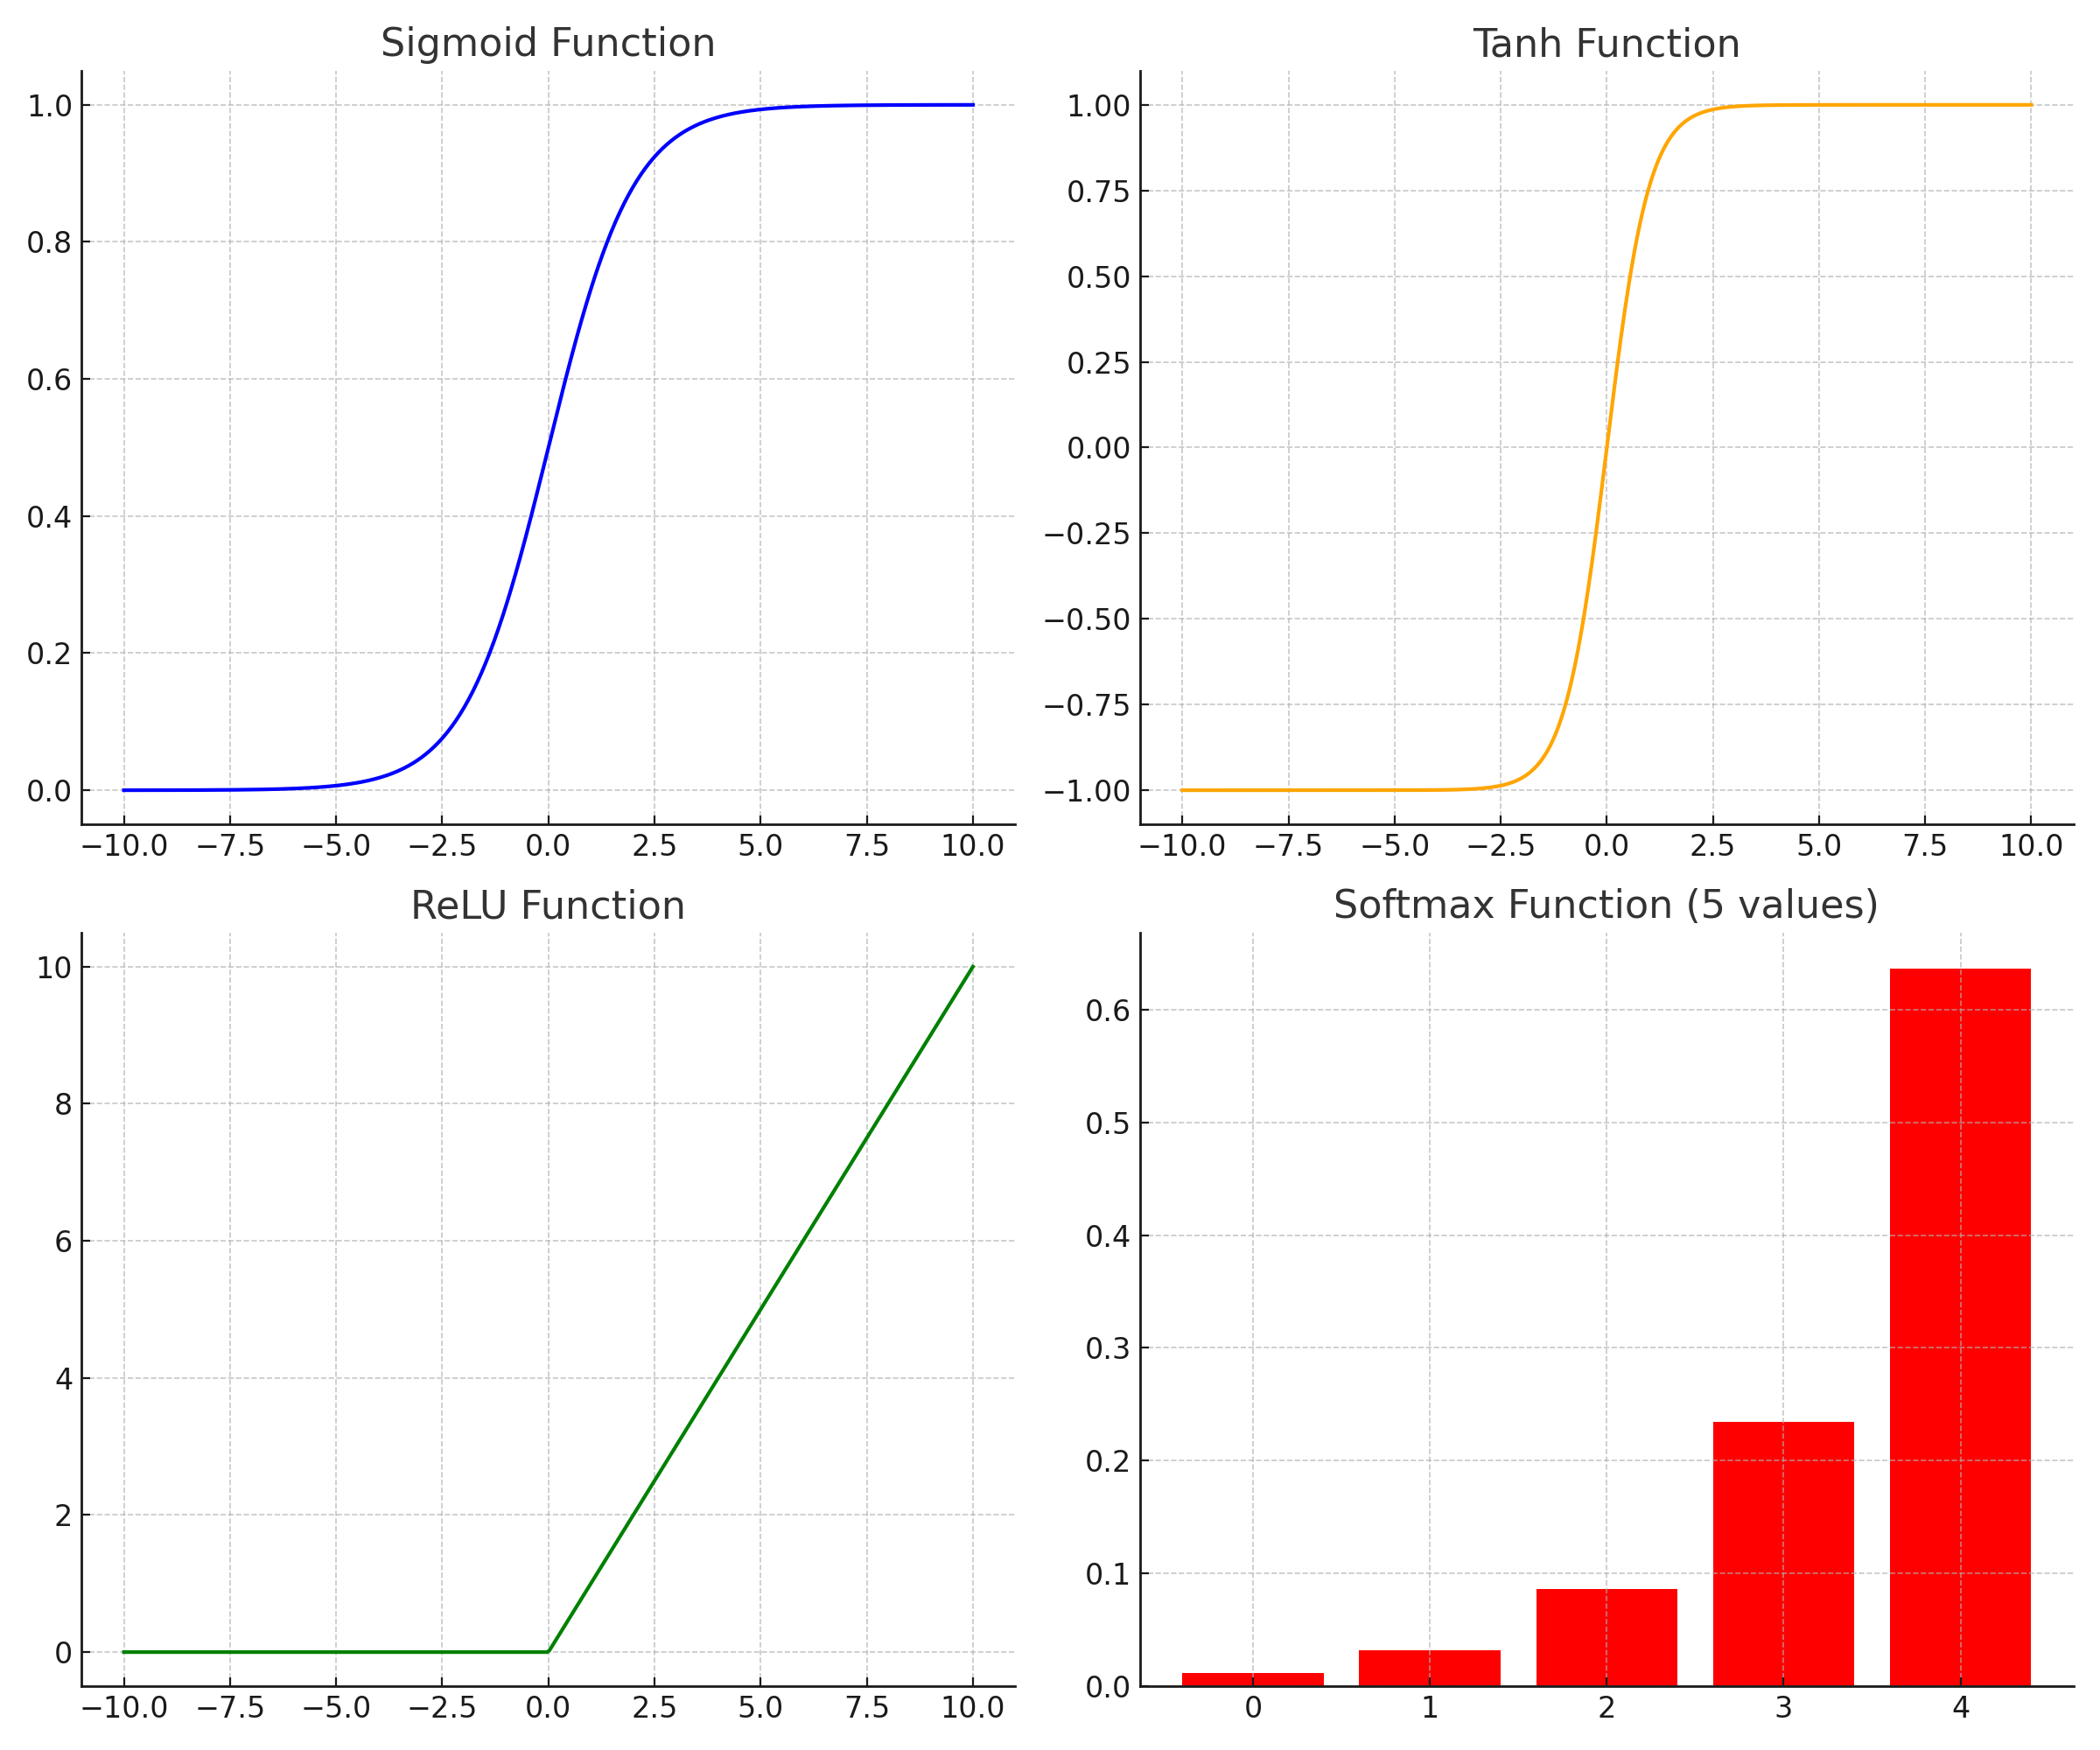
\includegraphics[width=0.9\textwidth]{assets/pics/activation_functions.png}}
    \caption{ Grafik fungsi aktivasi: (a) Sigmoid, (b) Tanh, (c) ReLU, dan (d) Softmax untuk
menunjukkan karakteristik output masing-masing fungsi}
    \source{Digenerate menggunakan Chat-GPT}
    \label{fig:activation_graph}
\end{figure}

%-----------------------------------------------------------------------------%
\section{Arsitektur Deep Learning untuk Computer Vision}
%-----------------------------------------------------------------------------%

\textit{Computer vision} merupakan domain yang telah mengalami transformasi revolusioner dengan kemunculan \textit{deep learning}. Arsitektur yang dirancang khusus untuk memproses data visual telah mencapai tingkat kinerja yang melampaui kemampuan manusia dalam banyak tugas. Dalam konteks deteksi \textit{deepfake}, pemilihan arsitektur yang tepat menjadi krusial karena setiap arsitektur memiliki bias induktif yang berbeda dalam memproses informasi visual.

\subsection{Convolutional Neural Networks (CNN)}

\textit{Convolutional Neural Networks} merepresentasikan terobosan fundamental dalam \textit{computer vision}, dirancang secara spesifik untuk mengatasi tantangan yang melekat dalam pemrosesan data visual \cite{lecun1998gradient}. Berbeda dengan jaringan \textit{fully connected} yang memperlakukan setiap piksel secara independen, CNN memanfaatkan struktur spasial dari citra melalui operasi konvolusi yang mempertahankan hubungan spasial antar piksel.

Inspirasi CNN berasal dari sistem visual biologis, khususnya konsep \textit{receptive fields} dimana neuron dalam korteks visual hanya merespons stimuli dalam wilayah spasial terbatas. Prinsip ini ditranslasikan menjadi operasi konvolusi dimana filter berukuran kecil (biasanya 3×3 atau 5×5 piksel) bergerak melintasi seluruh citra, mengekstrak fitur lokal pada setiap posisi.

Operasi konvolusi fundamental dapat diformulasikan sebagai:
\begin{equation}
(I * K)(i,j) = \sum_{m} \sum_{n} I(i+m, j+n) \cdot K(m,n)
\label{eq:convolution}
\end{equation}

dimana $I$ adalah citra masukan, $K$ adalah kernel/filter, dan $*$ mennotasikan operasi konvolusi. Setiap filter belajar mendeteksi pola spesifik seperti tepi, tekstur, atau bentuk.

\begin{figure}[H]
    \centering
    \fbox{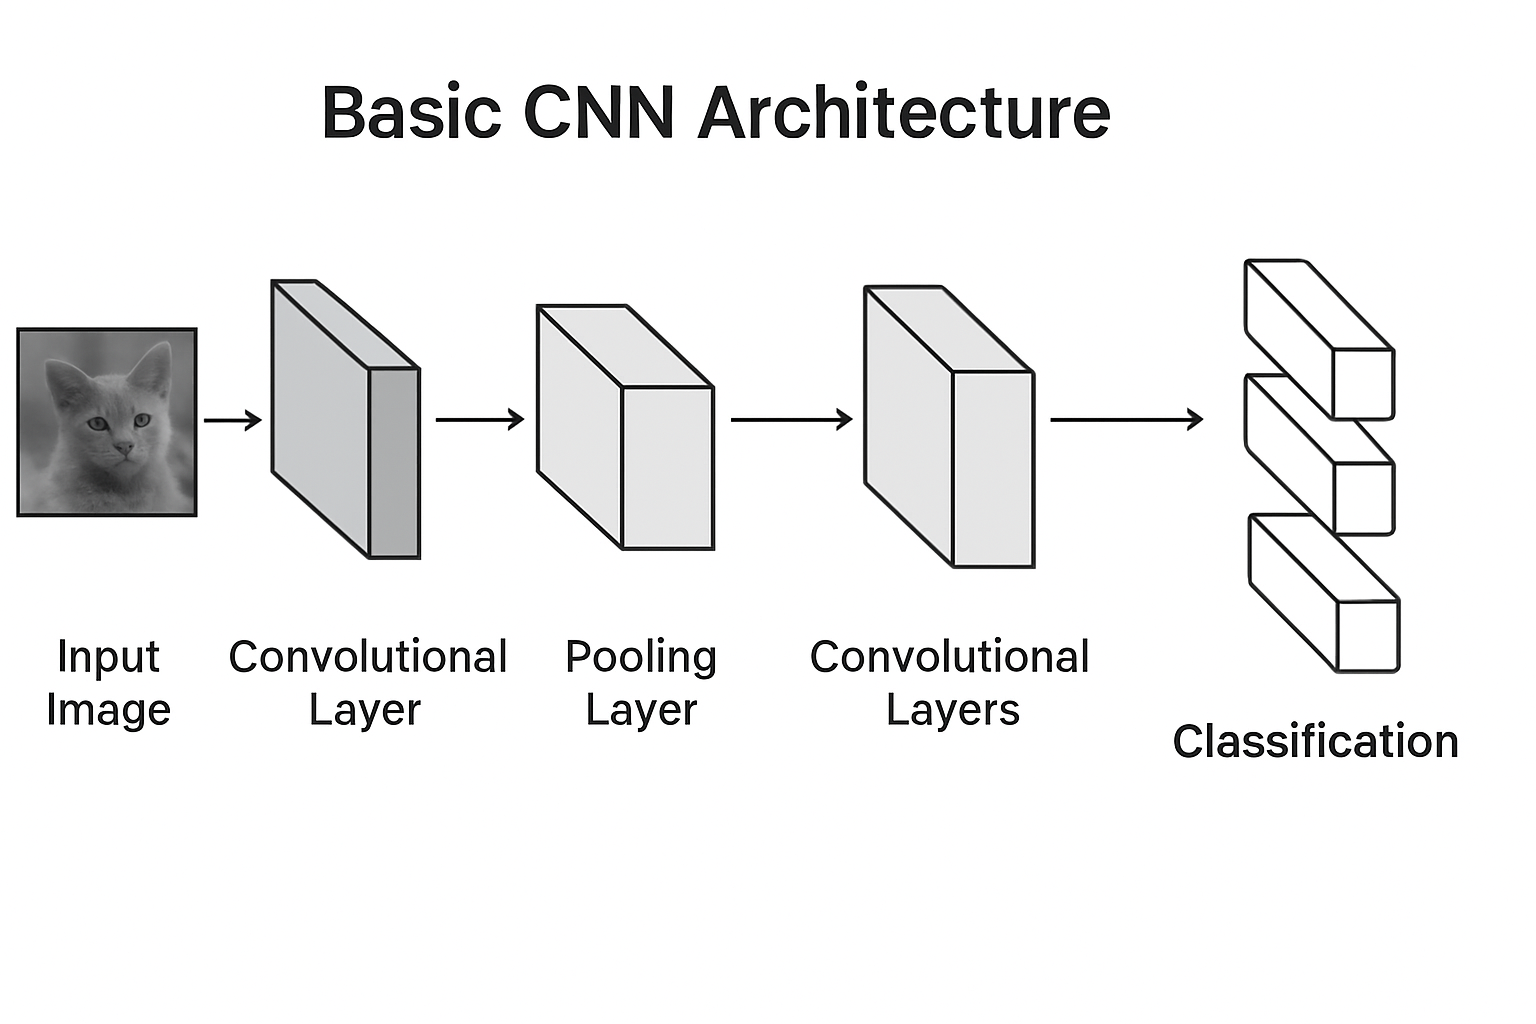
\includegraphics[width=0.9\textwidth]{assets/pics/cnn_architecture.png}}
    \caption{Arsitektur dasar CNN menunjukkan progres hierarkis dari fitur tingkat rendah ke representasi tingkat tinggi melalui lapisan konvolusi dan \textit{pooling} yang bergantian}
    \source{Diadaptasi dari \cite{lecun1998gradient}}
    \label{fig:cnn_architecture}
\end{figure}

Arsitektur CNN membangun representasi hierarkis melalui lapisan yang bergantian. \textit{Lapisan konvolusi} mengekstrak fitur lokal menggunakan filter yang dipelajari, dengan setiap filter mengkhususkan diri dalam mendeteksi pola tertentu. \textit{Lapisan pooling} mengurangi dimensi spasial sambil mempertahankan informasi penting, memberikan invariansi translasi dan efisiensi komputasi. \textit{Lapisan fully connected} pada akhir jaringan mengintegrasikan fitur yang diekstrak untuk keputusan klasifikasi akhir.

Keunggulan fundamental CNN dibandingkan jaringan \textit{fully connected} meliputi aspek-aspek krusial. \textit{Parameter sharing} memungkinkan filter yang sama digunakan di seluruh citra, secara dramatis mengurangi jumlah parameter yang perlu dipelajari. \textit{Translation invariance} memungkinkan deteksi fitur pada berbagai posisi dalam citra, krusial untuk pengenalan objek yang robust. \textit{Local connectivity} memastikan setiap neuron hanya terhubung ke wilayah spasial terbatas, menangkap pola lokal secara efektif. \textit{Hierarchical feature learning} membangun pemahaman progresif dari tepi dan tekstur tingkat rendah menuju konsep semantik tingkat tinggi.

Dalam konteks deteksi \textit{deepfake}, properti-properti ini sangat berharga karena artefak manipulasi dapat muncul pada berbagai skala dan lokasi dalam citra, dan pemrosesan hierarkis CNN dapat menangkap inkonsistensi pada berbagai tingkat abstraksi.

\subsection{Arsitektur CNN Modern}

Evolusi arsitektur CNN telah didorong oleh kebutuhan untuk mengatasi keterbatasan dari arsitektur sebelumnya sambil meningkatkan kinerja dan efisiensi. Setiap inovasi dalam arsitektur CNN modern mengatasi tantangan spesifik yang ditemukan dalam praktik, menciptakan ekosistem yang kaya dari pilihan arsitektur untuk berbagai aplikasi.

\subsubsection{ResNet: Revolusi Jaringan Dalam melalui Residual Learning}

\textit{Residual Network} (ResNet) merepresentasikan pergeseran paradigma fundamental dalam desain jaringan dalam, mengatasi salah satu hambatan utama dalam pelatihan jaringan yang sangat dalam: masalah \textit{vanishing gradient} \cite{he2016deep}. Sebelum ResNet, ada paradoks dimana menambahkan lebih banyak lapisan seharusnya tidak menurunkan kinerja (karena jaringan yang lebih dalam bisa mempelajari pemetaan identitas untuk lapisan tambahan), namun dalam praktik, jaringan yang sangat dalam sering menunjukkan degradasi kinerja.

ResNet mengatasi masalah ini melalui pengenalan kerangka \textit{residual learning}. Alih-alih mempelajari pemetaan langsung $H(x)$, blok residual belajar fungsi residual $F(x) = H(x) - x$, dengan keluaran akhir:

\begin{equation}
H(x) = F(x) + x
\label{eq:residual_output}
\end{equation}

Wawasan kunci adalah bahwa mempelajari residual lebih mudah daripada mempelajari transformasi lengkap, terutama ketika fungsi optimal mendekati pemetaan identitas.

\begin{figure}[H]
    \centering
    \fbox{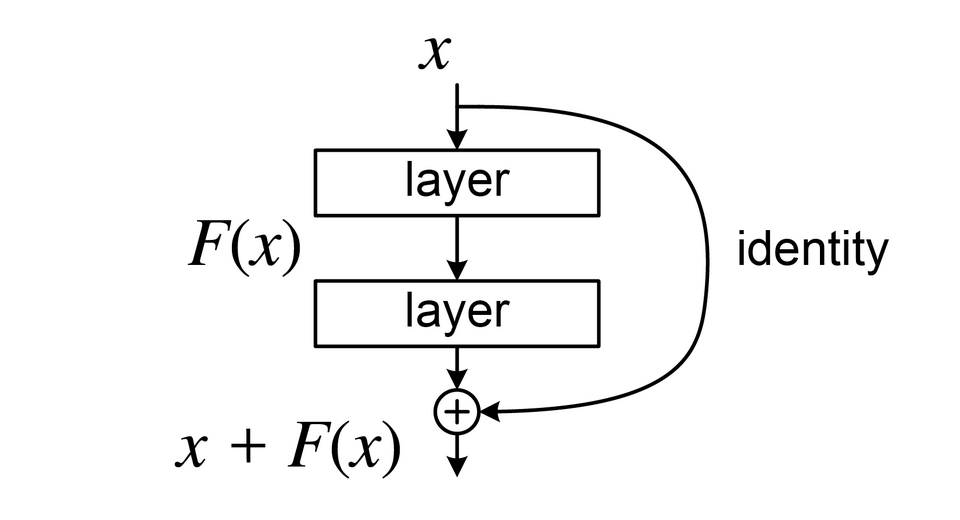
\includegraphics[width=0.6\textwidth]{assets/pics/resnet_block.png}}
    \caption{Arsitektur blok residual menunjukkan koneksi langsung yang memungkinkan aliran informasi dan propagasi gradien langsung melalui jalur pintas}
    \source{Diadaptasi dari \cite{he2016deep}}
    \label{fig:resnet_block}
\end{figure}

\textit{Skip connections} dalam ResNet berfungsi sebagai "jalan raya informasi" yang memungkinkan gradien mengalir langsung ke lapisan sebelumnya, mengurangi masalah \textit{vanishing gradient}. Hal ini memungkinkan pelatihan jaringan dengan ratusan atau bahkan ribuan lapisan, membuka kemungkinan untuk mempelajari representasi yang sangat kompleks.

Dalam konteks deteksi \textit{deepfake}, kemampuan ResNet untuk mempelajari representasi yang sangat dalam khususnya berharga karena artefak manipulasi yang halus mungkin memerlukan transformasi fitur yang kompleks untuk dideteksi secara efektif. Jaringan dalam dapat menangkap pola rumit yang mengindikasikan pembangkitan konten sintetis.

\subsubsection{Xception: Extreme Inception dan Depthwise Separable Convolutions}

\textit{Xception} merepresentasikan solusi elegan untuk efisiensi komputasi dalam desain CNN melalui interpretasi ekstrem dari hipotesis Inception \cite{chollet2017xception}. Inovasi inti terletak pada penggantian konvolusi standar dengan \textit{depthwise separable convolutions}, yang secara dramatis mengurangi biaya komputasi sambil mempertahankan atau bahkan meningkatkan kinerja.

Konvolusi standar secara simultan melakukan konvolusi spasial dan korelasi lintas saluran dalam operasi tunggal. Xception memisahkan dua operasi ini menjadi langkah berurutan yang lebih efisien. \textit{Depthwise separable convolution} memecah proses ini menjadi:

\textbf{Depthwise Convolution}: Mengaplikasikan filter spasial secara independen pada setiap saluran masukan, menangkap korelasi spasial dalam setiap saluran tanpa mencampur informasi lintas saluran.

\textbf{Pointwise Convolution}: Menggunakan konvolusi 1×1 untuk mengkombinasikan informasi lintas saluran, mempelajari kombinasi optimal saluran-wise dari fitur yang telah difilter spasial.

\begin{figure}[H]
    \centering
    \fbox{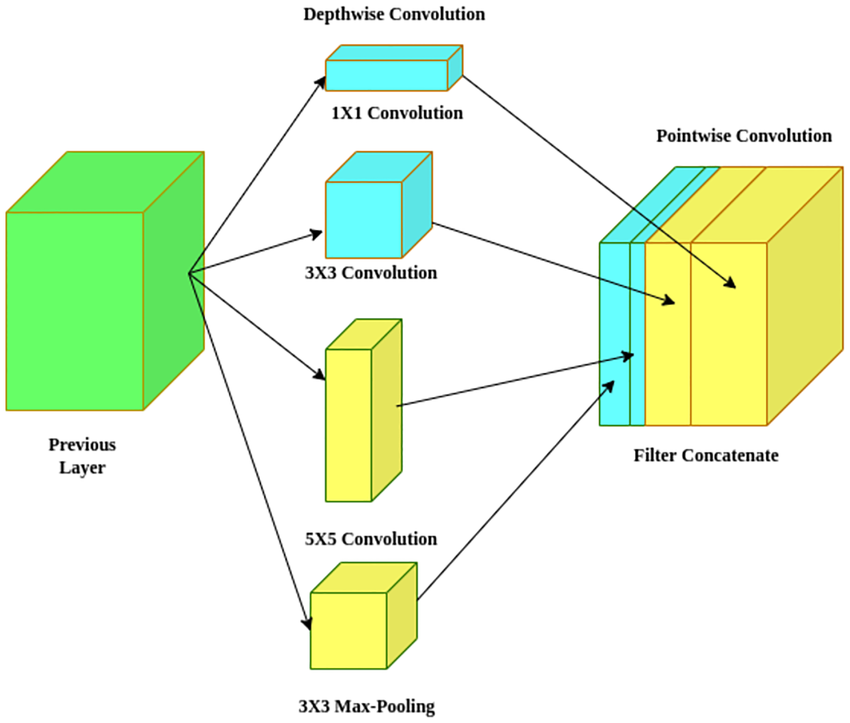
\includegraphics[width=0.8\textwidth]{assets/pics/xception_block.png}}
    \caption{Arsitektur Depthwise Separable Convolution menunjukkan pemisahan pemrosesan spasial dan saluran-wise untuk meningkatkan efisiensi}
    \source{Diadaptasi dari \cite{chollet2017xception}}
    \label{fig:xception_block}
\end{figure}

Pendekatan ini tidak hanya mengurangi kompleksitas komputasi secara signifikan (biasanya pengurangan 8-10x dalam multiply-adds) tetapi juga memberikan fleksibilitas pemodelan. Pemisahan pemrosesan spasial dan saluran memungkinkan jaringan untuk secara independen mengoptimalkan ekstraksi fitur spasial dan pencampuran saluran, berpotensi mengarah ke representasi fitur yang lebih baik.

Untuk deteksi \textit{deepfake}, pemrosesan efisien Xception khususnya menguntungkan karena memungkinkan penerapan model canggih dengan batasan komputasi, sambil mempertahankan sensitivitas tinggi untuk mendeteksi artefak manipulasi yang halus.

\subsubsection{EfficientNet: Penskalaan Berprinsip untuk Kinerja Optimal}

\textit{EfficientNet} mengatasi pertanyaan fundamental dalam desain CNN: bagaimana cara optimal untuk menskala jaringan untuk kinerja yang lebih baik \cite{tan2019efficientnet}. Pendekatan tradisional fokus pada penskalaan dimensi tunggal - membuat jaringan lebih dalam (lebih banyak lapisan), lebih lebar (lebih banyak saluran), atau memproses masukan resolusi lebih tinggi. EfficientNet memperkenalkan \textit{compound scaling} yang secara sistematis menyeimbangkan ketiga dimensi.

Wawasan inti adalah bahwa ketiga dimensi penskalaan saling bergantung. Meningkatkan resolusi masukan memerlukan lebih banyak lapisan untuk menangkap pola detail, dan lebih banyak saluran untuk menangkap kepadatan informasi yang meningkat. \textit{Compound scaling} mengkoordinasikan penskalaan di semua dimensi menggunakan pendekatan berprinsip:

\begin{align}
\text{kedalaman} &= \alpha^\phi \label{eq:depth_scaling} \\
\text{lebar} &= \beta^\phi \label{eq:width_scaling} \\
\text{resolusi} &= \gamma^\phi \label{eq:resolution_scaling}
\end{align}

dengan batasan yang memastikan biaya komputasi total berskala secara dapat diprediksi: $\alpha \cdot \beta^2 \cdot \gamma^2 \approx 2$

Koefisien $\alpha$, $\beta$, dan $\gamma$ ditentukan melalui pencarian grid sistematis pada jaringan dasar, kemudian $\phi$ digunakan sebagai koefisien majemuk untuk memperbesar jaringan secara seragam.

\begin{figure}[H]
    \centering
    \fbox{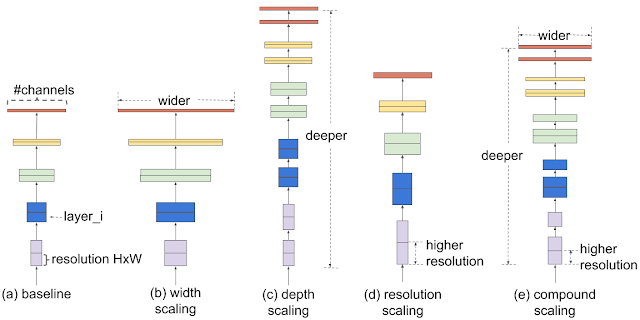
\includegraphics[width=0.9\textwidth]{assets/pics/efficientnet_scaling.png}}
    \caption{Perbandingan strategi penskalaan menunjukkan superioritas compound scaling dalam mencapai tradeoff akurasi-efisiensi yang optimal}
    \source{Diadaptasi dari \cite{tan2019efficientnet}}
    \label{fig:efficientnet_scaling}
\end{figure}

Hasil dari pendekatan ini adalah keluarga model yang secara konsisten mencapai akurasi \textit{state-of-the-art} dengan parameter dan FLOP yang signifikan lebih sedikit dibandingkan pendekatan penskalaan tradisional. EfficientNet menunjukkan bahwa perhatian yang cermat terhadap strategi penskalaan dapat menghasilkan peningkatan dramatis dalam efisiensi tanpa mengorbankan kinerja.

Dalam aplikasi deteksi \textit{deepfake}, pendekatan seimbang EfficientNet khususnya berharga karena memberikan tradeoff optimal antara akurasi deteksi dan efisiensi komputasi, memungkinkan penerapan dalam skenario praktis dengan batasan sumber daya.

%-----------------------------------------------------------------------------%
\section{Ensemble Learning dan Weighted Averaging}
%-----------------------------------------------------------------------------%

\textit{Ensemble learning} merepresentasikan salah satu paradigma paling powerful dalam \textit{machine learning}, berdasarkan intuisi fundamental bahwa kombinasi dari beberapa prediktor independen seringkali superior dibandingkan prediktor individual manapun. Prinsip ini, yang dikenal sebagai \textit{"wisdom of crowds"}, telah terbukti efektif di berbagai aplikasi dan khususnya relevan untuk tugas yang menantang seperti deteksi \textit{deepfake} dimana model tunggal mungkin memiliki bias atau titik buta \cite{dietterich2000ensemble}.

\subsection{Prinsip Dasar dan Fondasi Teoritis}

Fondasi teoritis dari \textit{ensemble learning} berakar pada teori pembelajaran statistik, khususnya konsep dekomposisi bias-varians. Pemahaman ini krusial untuk mengapresiasi mengapa metode ensemble bekerja dan kapan mereka diharapkan memberikan peningkatan dibanding model individual.

Keberhasilan ensemble dapat dijelaskan melalui lensa \textit{bias-variance tradeoff} \cite{breiman1996bias}. Untuk tugas regresi, galat yang diharapkan dari prediktor dapat didekomposisi menjadi tiga komponen: bias (galat sistematis dari asumsi yang salah), varians (sensitivitas terhadap fluktuasi kecil dalam set pelatihan), dan galat yang tidak dapat direduksi (noise yang melekat dalam masalah).

Ketika kita mengkombinasikan beberapa model yang dilatih pada data berbeda atau dengan algoritma berbeda, ensemble dapat secara simultan mengurangi varians tanpa harus meningkatkan bias. Untuk ensemble dari $M$ model yang tidak berkorelasi dengan varians yang sama $\sigma^2$, varians dari prediksi ensemble berkurang menjadi:

\begin{equation}
\text{Var}[\bar{f}(x)] = \frac{\sigma^2}{M}
\label{eq:ensemble_variance}
\end{equation}

Pengurangan ini powerful, tetapi efektivitasnya sangat bergantung pada diversitas antar anggota ensemble. Jika model sangat berkorelasi (membuat kesalahan serupa), manfaat dari ensembling berkurang signifikan.

\textbf{Diversitas} merupakan kunci keberhasilan \textit{ensemble learning}. Model yang berbeda cenderung membuat kesalahan yang berbeda pada instans yang berbeda, dan ketika galat tidak berkorelasi atau berkorelasi negatif, mereka dapat saling membatalkan ketika dikombinasikan. Dalam konteks deteksi \textit{deepfake}, arsitektur CNN yang berbeda menangkap jenis informasi visual dan artefak yang berbeda, menciptakan diversitas alami yang menguntungkan untuk kinerja ensemble.

\begin{figure}[H]
    \centering
    \fbox{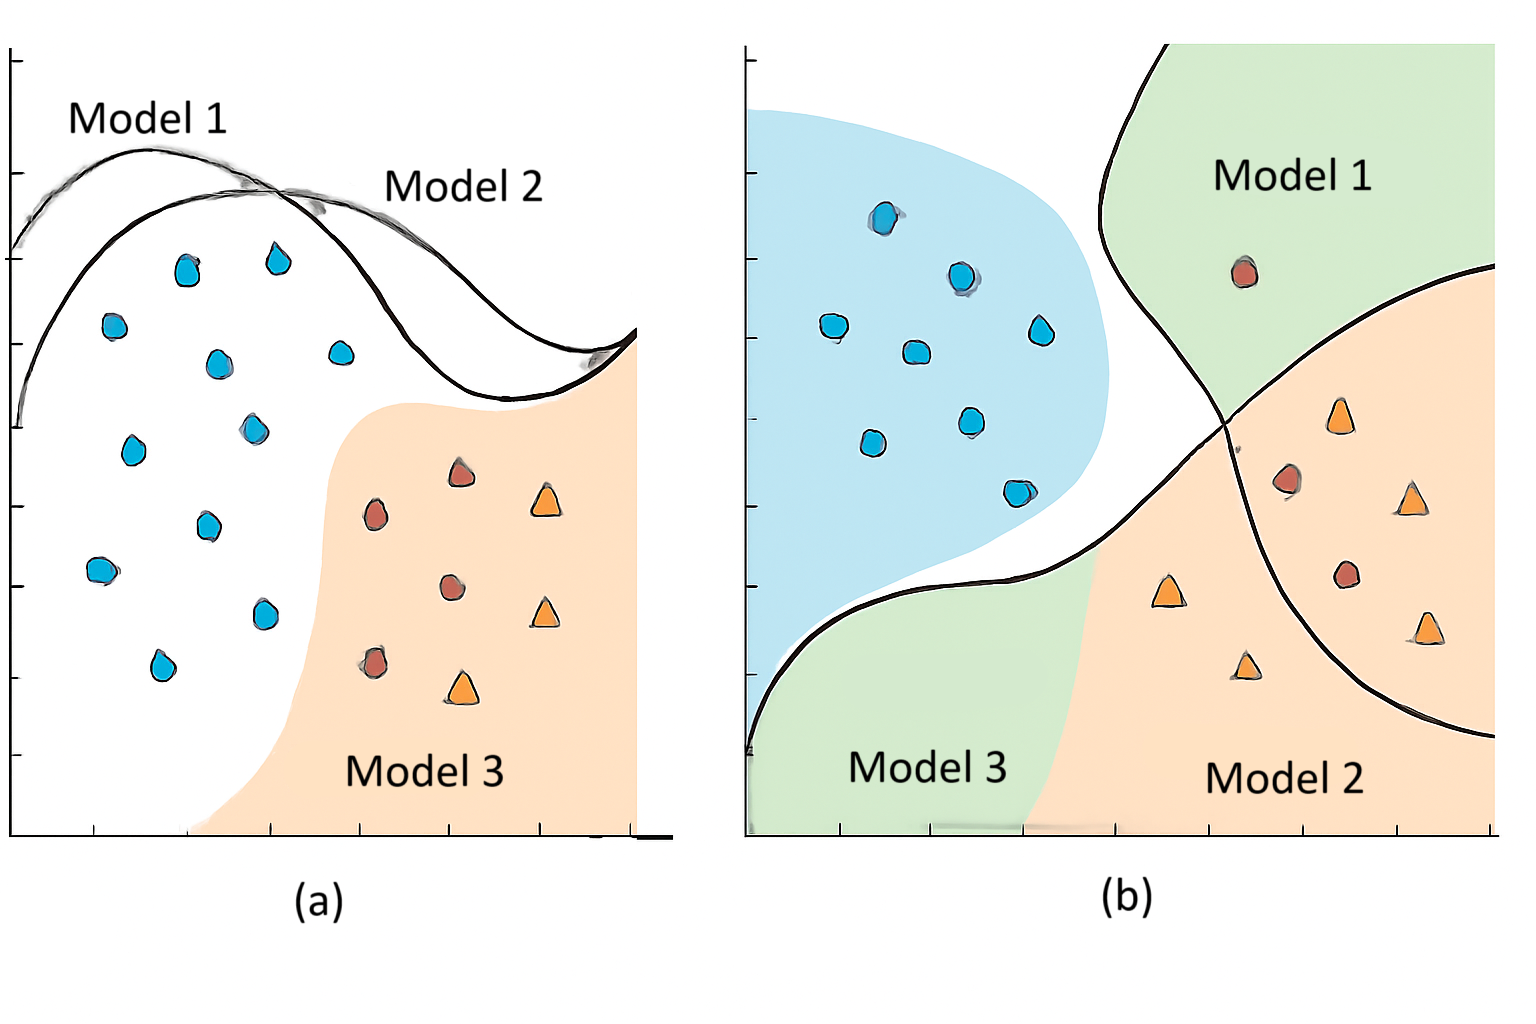
\includegraphics[width=0.8\textwidth]{assets/pics/ensemble_diversity.png}}
    \caption{Visualisasi efek diversitas ensemble: pola galat yang beragam memungkinkan koreksi galat mutual, sementara pola galat yang serupa memberikan manfaat ensemble yang minimal}
    \source{Ilustrasi berdasarkan \cite{brown2005diversity}}
    \label{fig:ensemble_diversity}
\end{figure}

Diversitas dapat diukur melalui berbagai metrik. Q-statistic mengukur tingkat kesepakatan antar classifier, ukuran ketidaksepakatan menghitung proporsi instans dimana classifier tidak setuju, dan ukuran kesalahan ganda mengukur proporsi instans dimana kedua classifier salah. Ensemble optimal menyeimbangkan akurasi individual dengan diversitas antar model.

\subsection{Metode Ensemble Learning: Tinjauan Komprehensif}

Lanskap metode ensemble kaya dan beragam, dengan setiap pendekatan menargetkan aspek berbeda dari konstruksi dan kombinasi ensemble. Memahami paradigma ensemble yang berbeda esensial untuk memilih metode yang tepat untuk aplikasi spesifik.

\subsubsection{Bagging: Bootstrap Aggregating untuk Pengurangan Varians}

\textit{Bootstrap Aggregating} (Bagging) mengatasi komponen varians dari galat prediksi melalui pelatihan beberapa model pada sampel bootstrap yang berbeda dari data pelatihan \cite{breiman1996bagging}. Pendekatan ini khususnya efektif untuk model dengan varians tinggi seperti \textit{decision trees}, tetapi juga dapat diterapkan untuk jaringan saraf.

Ide inti di balik bagging adalah bahwa merata-ratakan prediksi dari beberapa model yang dilatih pada dataset yang sedikit berbeda dapat mengurangi varians keseluruhan tanpa secara signifikan mempengaruhi bias. \textit{Bootstrap sampling} menciptakan set pelatihan yang beragam dengan mengambil sampel ulang data asli dengan penggantian, memastikan bahwa setiap model melihat versi data yang sedikit berbeda.

Proses dimulai dengan menghasilkan $M$ sampel bootstrap, masing-masing berukuran sama dengan set pelatihan asli tetapi dengan komposisi berbeda karena pengambilan sampel dengan penggantian. Setiap sampel bootstrap kemudian digunakan untuk melatih model terpisah. Prediksi akhir diperoleh melalui perata-rataan (untuk regresi) atau \textit{majority voting} (untuk klasifikasi):

\begin{equation}
\hat{y} = \text{mode}\{h_1(x), h_2(x), \ldots, h_M(x)\}
\label{eq:bagging_prediction}
\end{equation}

Bagging khususnya efektif ketika model dasar rentan terhadap \textit{overfitting}, karena efek perata-rataan menghaluskan keanehan model individual. Dalam konteks \textit{deep learning}, bagging dapat diterapkan dengan melatih arsitektur yang sama pada subset data yang berbeda atau dengan inisialisasi acak yang berbeda.

\subsubsection{Boosting: Pembelajaran Berurutan dengan Fokus Galat}

\textit{Boosting} mengambil pendekatan yang secara fundamental berbeda dibandingkan bagging, fokus pada pengurangan bias melalui proses pelatihan berurutan dimana setiap model berikutnya fokus pada memperbaiki galat yang dibuat oleh model sebelumnya \cite{freund1997decision}. Ini menciptakan proses pembelajaran adaptif yang secara progresif meningkatkan kinerja pada instans yang sulit.

\textit{AdaBoost} (Adaptive Boosting) merupakan algoritma boosting seminal yang mengilustrasikan prinsip inti. Algoritma mempertahankan bobot untuk setiap instans pelatihan, awalnya diatur sama. Setelah melatih setiap \textit{weak learner}, bobot instans diperbarui: instans yang diklasifikasikan dengan benar menerima bobot yang lebih rendah, sementara instans yang salah diklasifikasikan menerima bobot yang lebih tinggi. Skema pembobotan ini memastikan bahwa \textit{learner} berikutnya memfokuskan perhatian pada instans yang sebelumnya sulit.

Sifat berurutan dari boosting menciptakan kombinasi yang kuat dimana ensemble akhir menggabungkan \textit{weak learner} secara berbobot, dengan performer yang lebih baik menerima pengaruh yang lebih tinggi dalam keputusan akhir. Formulasi matematis memastikan bahwa galat pelatihan menurun secara eksponensial dengan jumlah putaran boosting, di bawah kondisi yang tepat.

Namun, boosting dapat rentan terhadap \textit{overfitting} dan noise, terutama dengan model yang sangat dalam seperti CNN. Regularisasi yang hati-hati dan \textit{early stopping} seringkali diperlukan ketika menerapkan prinsip boosting untuk aplikasi \textit{deep learning}.

\subsubsection{Stacking: Meta-Learning untuk Kombinasi Optimal}

\textit{Stacking} (Stacked Generalization) merepresentasikan pendekatan canggih untuk kombinasi ensemble melalui pengenalan \textit{meta-learner} yang mempelajari cara optimal untuk mengkombinasikan prediksi model dasar \cite{wolpert1992stacked}. Tidak seperti bagging atau boosting yang menggunakan aturan kombinasi sederhana, stacking mempelajari fungsi kombinasi dari data.

Arsitektur terdiri dari dua tingkat: \textit{Level-0 base learners} dilatih pada data asli, dan \textit{Level-1 meta-learner} dilatih untuk mengkombinasikan prediksi Level-0. Proses biasanya melibatkan \textit{cross-validation} untuk menghasilkan meta-fitur: model dasar dilatih pada subset data digunakan untuk menghasilkan prediksi untuk bagian yang ditahan, menciptakan set pelatihan untuk \textit{meta-learner}.

Stacking khususnya powerful karena \textit{meta-learner} dapat mempelajari kombinasi non-linear yang kompleks dari prediksi dasar, berpotensi menemukan efek interaksi dan kekuatan komplementer antar model dasar. Namun, kompleksitas pendekatan stacking memerlukan validasi yang hati-hati untuk menghindari \textit{overfitting}, terutama dengan data pelatihan yang terbatas.

\subsection{Weighted Averaging: Kesederhanaan Elegan dengan Efektivitas Terbukti}

\textit{Weighted averaging} merepresentasikan titik manis dalam metodologi ensemble - cukup canggih untuk menangkap kinerja diferensial antar model dasar, namun cukup sederhana untuk diimplementasikan secara andal dan diinterpretasikan secara bermakna \cite{kuncheva2004combining}. Metode ini memberikan bobot berbeda kepada prediksi model dasar berdasarkan estimasi kinerja, menciptakan kombinasi bernuansa yang memanfaatkan kekuatan model yang lebih baik sambil tetap mendapat manfaat dari diversitas model yang lebih lemah.

Formulasi matematis yang sederhana namun powerful:
\begin{equation}
\hat{y}_{ensemble}(x) = \sum_{i=1}^{N} w_i \cdot \hat{y}_i(x)
\label{eq:weighted_ensemble}
\end{equation}

dengan batasan fundamental: $\sum_{i=1}^{N} w_i = 1$ dan $w_i \geq 0$. Batasan ini memastikan bahwa keluaran ensemble tetap dalam batas yang wajar dan bahwa semua model berkontribusi secara non-negatif.

\textbf{Strategi Pembobotan Berbasis Kinerja} yang diadopsi dalam penelitian ini memberikan bobot proporsional terhadap kinerja validasi:
\begin{equation}
w_i = \frac{\text{performance}_i}{\sum_{j=1}^{N} \text{performance}_j}
\label{eq:performance_weight}
\end{equation}

Pendekatan ini intuitif dan praktis efektif: model yang menunjukkan kinerja superior pada data validasi menerima pengaruh yang sesuai lebih tinggi dalam keputusan ensemble. Strategi ini mengasumsikan bahwa kinerja validasi prediktif terhadap kinerja tes, asumsi yang wajar ketika set validasi representatif dari distribusi target.

\begin{figure}[H]
    \centering
    \fbox{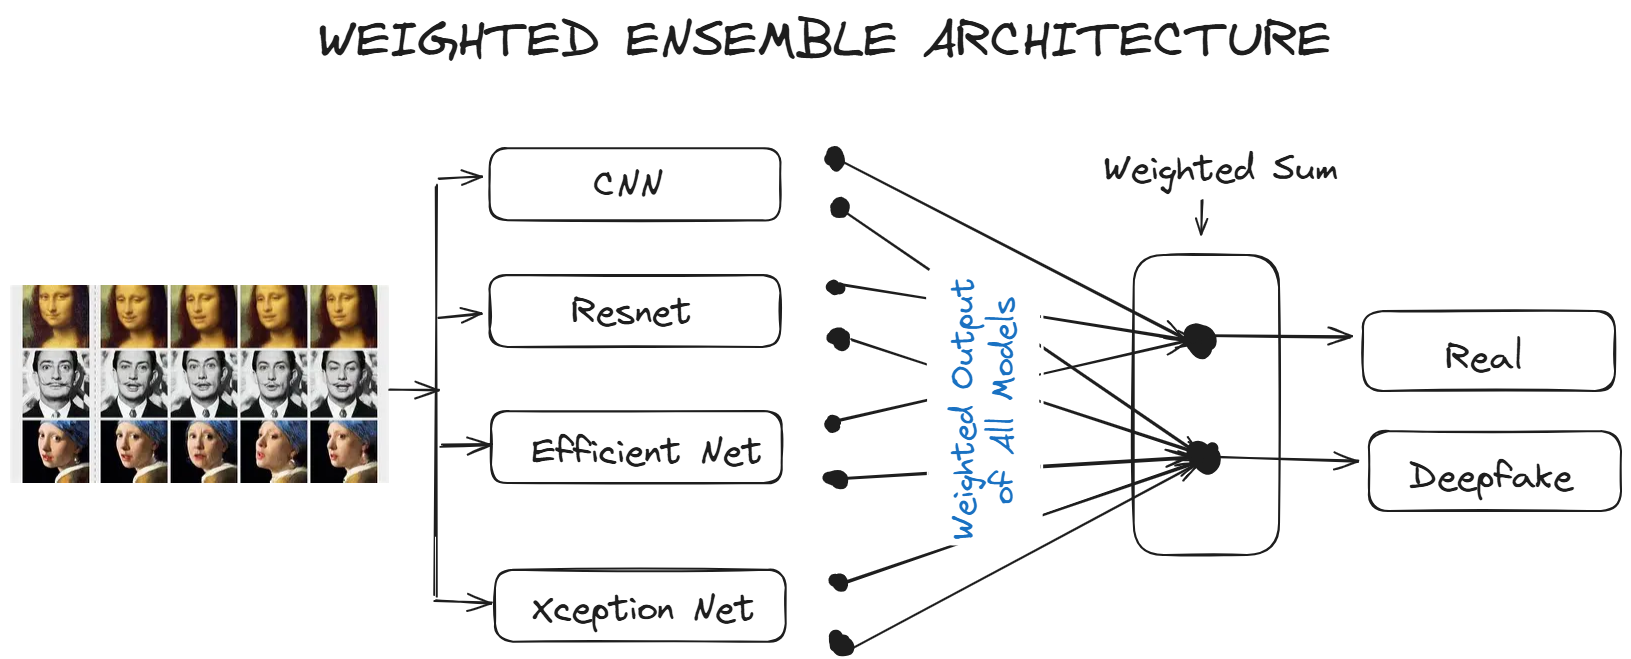
\includegraphics[width=0.9\textwidth]{assets/pics/weighted_ensemble.png}}
    \caption{Arsitektur ensemble berbobot menunjukkan aliran informasi dari masukan melalui beberapa model dasar, kombinasi berbobot, dan prediksi akhir}
    \source{Ilustrasi berdasarkan metodologi penelitian}
    \label{fig:weighted_ensemble}
\end{figure}

Keunggulan \textit{weighted averaging} meliputi beberapa aspek krusial. \textbf{Kesederhanaan komputasi} memungkinkan implementasi efisien tanpa prosedur pelatihan yang kompleks. \textbf{Interpretabilitas} memungkinkan pemahaman mudah tentang kontribusi setiap model terhadap keputusan akhir. \textbf{Fleksibilitas} dalam pemberian bobot memungkinkan adaptasi terhadap metrik kinerja yang berbeda atau persyaratan spesifik domain. \textbf{Robustness} terhadap kegagalan model individual, karena model dengan kinerja buruk secara otomatis menerima pengaruh yang lebih rendah.

Dalam konteks deteksi \textit{deepfake}, \textit{weighted averaging} khususnya cocok karena arsitektur CNN yang berbeda menunjukkan kinerja yang bervariasi pada jenis artefak manipulasi yang berbeda. Pemberian bobot berdasarkan akurasi validasi memastikan bahwa model dengan kemampuan deteksi superior memberikan pengaruh yang tepat pada keputusan ensemble akhir.

%-----------------------------------------------------------------------------%
\section{Teknologi Deepfake dan Deteksi}
%-----------------------------------------------------------------------------%

Era digital modern telah menyaksikan kemunculan teknologi manipulasi media canggih yang menantang konsep tradisional tentang kebenaran visual. Teknologi \textit{deepfake}, yang menggabungkan kekuatan \textit{deep learning} dengan aksesibilitas alat tingkat konsumen, merepresentasikan pergeseran paradigma dalam lanskap pembuatan dan manipulasi media digital. Memahami teknologi ini - baik dalam kemampuan maupun keterbatasannya - esensial untuk mengembangkan langkah-langkah perlawanan yang efektif.

\subsection{Teknologi Deepfake: Evolusi dan Keadaan Saat Ini}

Teknologi \textit{deepfake}, nama yang berasal dari penggabungan "\textit{deep learning}" dan "\textit{fake}", merepresentasikan konvergensi dari beberapa kemajuan teknologi dalam kecerdasan buatan, \textit{computer vision}, dan pemrosesan media \cite{rana2022deepfake}. Teknologi ini secara fundamental memanfaatkan kekuatan \textit{Generative Adversarial Networks} (GANs) untuk menciptakan konten media sintetis yang sangat realistis, khususnya untuk aplikasi penukaran wajah dan reenaktmen wajah.

Lintasan historis teknologi \textit{deepfake} luar biasa dalam kecepatan perkembangan yang pesat. Teknologi pertama kali mendapat perhatian luas pada akhir 2017 ketika pengguna Reddit dengan nama pengguna "deepfakes" merilis kode sumber terbuka untuk penukaran wajah menggunakan framework \textit{deep learning} yang tersedia \cite{ajder2019deepfakes}. Implementasi awal masih kasar, menghasilkan hasil dengan artefak yang jelas dan memerlukan keahlian teknis yang substansial untuk penerapan.

Perkembangan teknologi ini dapat ditelusuri melalui fase evolusi yang berbeda. Sistem \textbf{Generasi 1} berbasis pada arsitektur autoencoder sederhana, menghasilkan keluaran resolusi rendah dengan artefak visual yang jelas. \textbf{Generasi 2} memperkenalkan pendekatan berbasis GAN dengan peningkatan kualitas yang signifikan, memungkinkan pembuatan konten palsu yang lebih meyakinkan. Sistem \textbf{Generasi 3} memanfaatkan arsitektur canggih seperti StyleGAN dan teknik \textit{progressive growing}, mencapai kualitas yang mendekati fotorealistis. Sistem \textbf{Generasi 4} saat ini memungkinkan generasi real-time dan reenaktmen wajah dengan persyaratan komputasi minimal.

Teknologi \textit{deepfake} kontemporer menunjukkan kemampuan canggih yang mencakup beberapa modalitas. Sistem reenaktmen wajah dapat memanipulasi ekspresi wajah dan gerakan kepala secara real-time, memungkinkan peniruan yang meyakinkan untuk panggilan video atau live stream. Teknologi sintesis suara dapat mereplikasi pola bicara dengan fidelitas yang luar biasa menggunakan jumlah audio target yang relatif kecil. Sistem puppeteering seluruh tubuh dapat mentransfer gerakan dan gestur tubuh, menciptakan kemampuan peniruan yang komprehensif.

\textbf{Aplikasi Positif} dari teknologi \textit{deepfake} menunjukkan potensi signifikan untuk penggunaan yang bermanfaat. Industri hiburan memanfaatkan teknologi untuk kebangkitan digital aktor yang telah meninggal, memungkinkan penyelesaian film atau pembuatan konten baru yang menampilkan performer terkasih. Aplikasi pendidikan termasuk simulasi tokoh sejarah, memungkinkan siswa berinteraksi dengan representasi virtual dari kepribadian sejarah penting. Aplikasi aksesibilitas menyediakan sintesis suara untuk individu dengan gangguan bicara, memulihkan kemampuan komunikasi. Seni kreatif mendapat manfaat dari penangkapan kinerja yang ditingkatkan dan pembuatan avatar digital.

Namun, \textbf{risiko dan ancaman} yang terkait dengan teknologi \textit{deepfake} sama signifikan dan mengkhawatirkan. Kampanye disinformasi dapat memanfaatkan konten palsu yang realistis untuk manipulasi politik atau serangan rekayasa sosial. Aplikasi penipuan identitas memungkinkan peniruan yang tidak sah untuk penipuan keuangan atau kerusakan reputasi. Pelanggaran privasi melalui pembuatan citra intim tanpa persetujuan merepresentasikan kekhawatiran etis dan hukum yang serius. Serangan rekayasa sosial yang ditingkatkan dapat memanfaatkan peniruan yang meyakinkan untuk spionase korporat atau manipulasi personal.

\begin{figure}[H]
    \centering
    \fbox{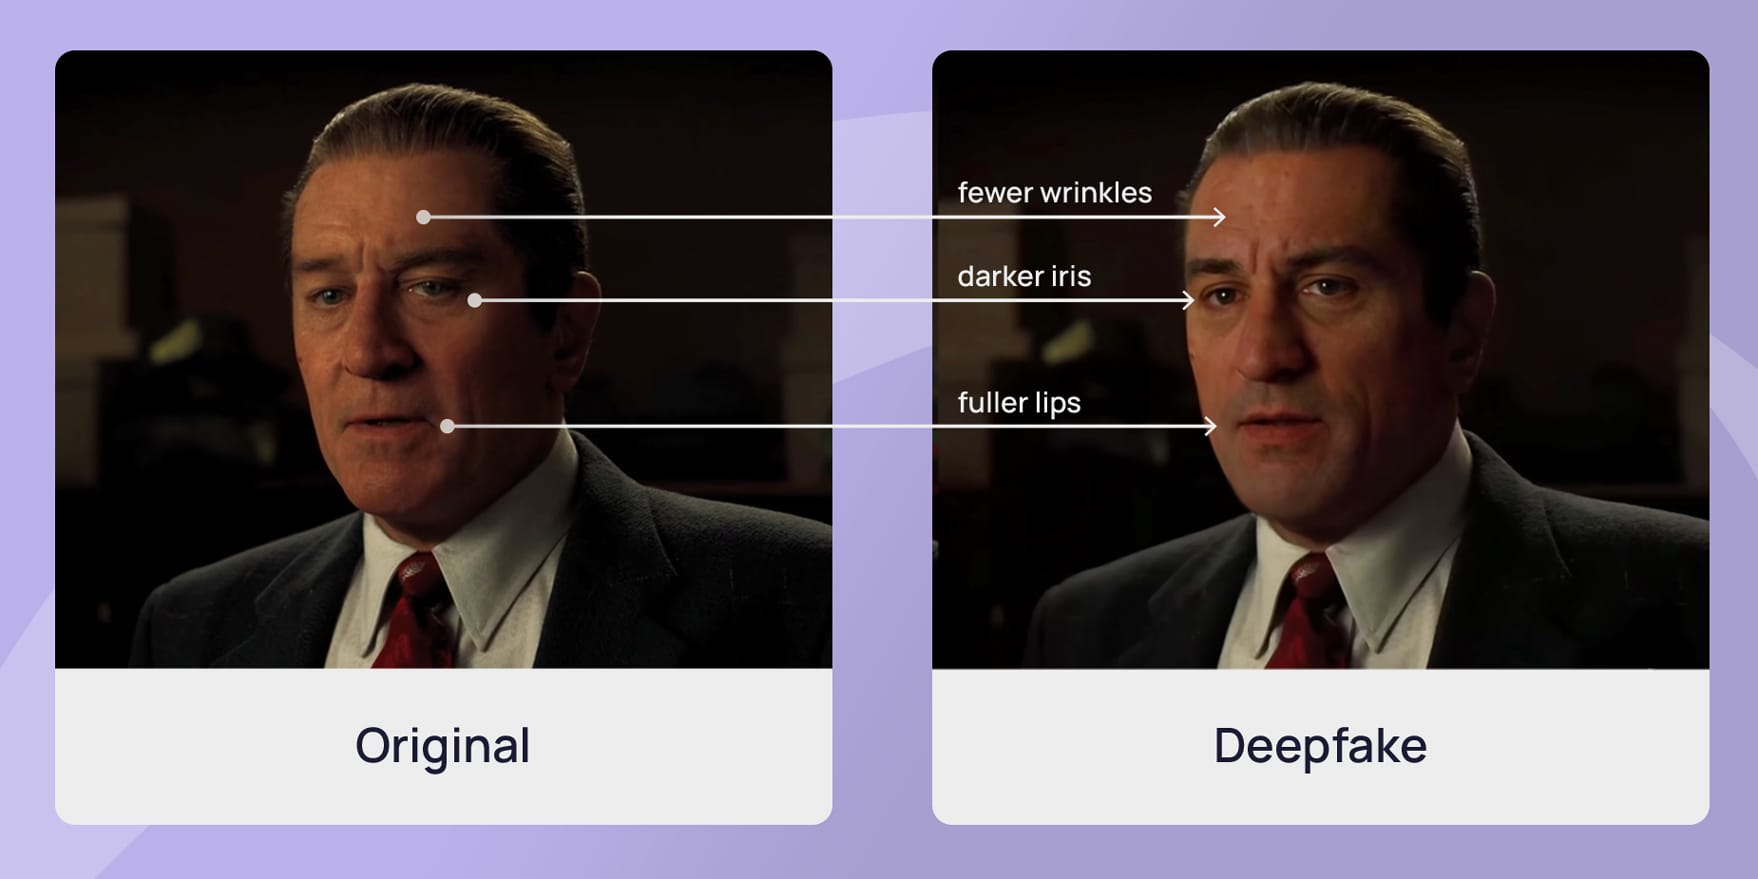
\includegraphics[width=0.9\textwidth]{assets/pics/deepfake_examples.jpg}}
    \caption{Pengaplikasian Deepfake}
    \source{Sumber: DQLab}
    \label{fig:deepfake_examples}
\end{figure}

\subsection{Generative Adversarial Networks: Mesin Pembuatan Media Sintetis}

\textit{Generative Adversarial Networks} merupakan fondasi teknologi yang memungkinkan pembuatan \textit{deepfake} canggih, merepresentasikan terobosan dalam pemodelan generatif yang merevolusi kemampuan untuk menciptakan konten sintetis \cite{goodfellow2014generative}. Memahami arsitektur dan dinamika pelatihan GAN krusial untuk memahami baik kemampuan maupun potensi kerentanan teknologi \textit{deepfake}.

Kerangka GAN terdiri dari dua jaringan saraf yang terlibat dalam proses pelatihan adversarial: jaringan generator yang berusaha menciptakan konten sintetis yang realistis, dan jaringan discriminator yang mencoba membedakan antara konten nyata dan yang dihasilkan. Hubungan adversarial ini menciptakan lingkungan pelatihan dinamis dimana kedua jaringan terus meningkat sebagai respons terhadap kemampuan lawan.

Formulasi matematis inti dari tujuan pelatihan GAN menangkap esensi hubungan adversarial:
\begin{equation}
\min_G \max_D V(D,G) = \mathbb{E}_{x \sim p_{data}}[\log D(x)] + \mathbb{E}_{z \sim p_z}[\log(1-D(G(z)))]
\label{eq:gan_objective}
\end{equation}

Discriminator memaksimalkan kemampuan untuk mengklasifikasikan sampel nyata dan palsu dengan benar, sementara generator meminimalkan akurasi klasifikasi discriminator. Proses pelatihan berlanjut hingga keseimbangan Nash tercapai, secara teoritis menghasilkan generator yang menghasilkan sampel yang tidak dapat dibedakan dari data nyata.

\begin{figure}[H]
    \centering
    \fbox{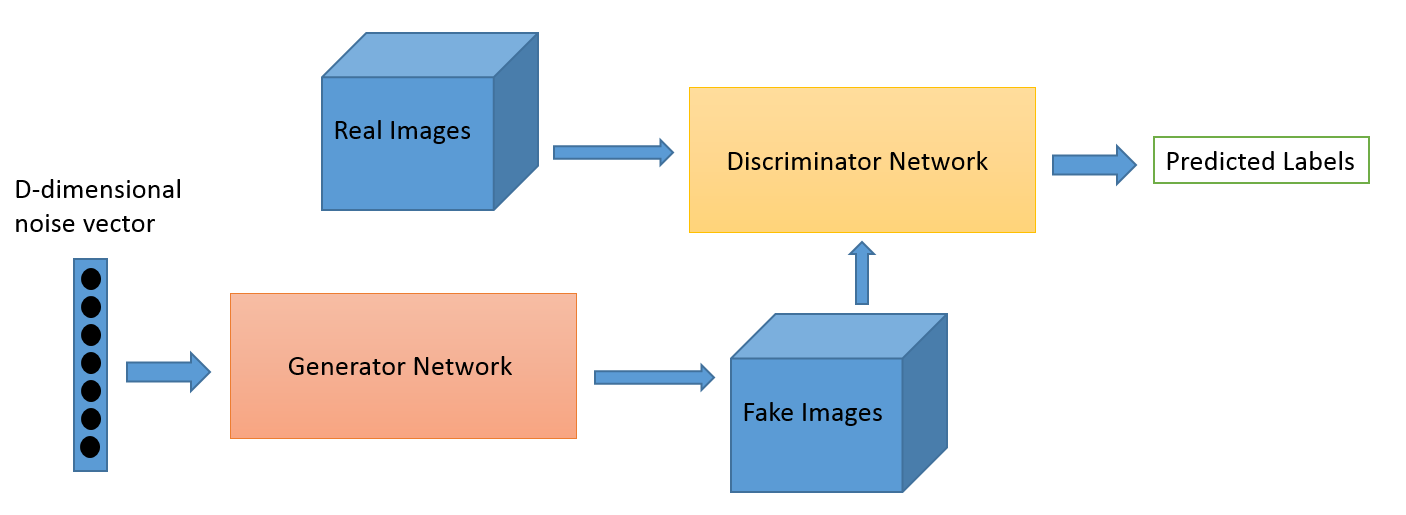
\includegraphics[width=0.9\textwidth]{assets/pics/gan_architecture.png}}
    \caption{Tinjauan arsitektur GAN menunjukkan setup pelatihan adversarial: (a) Fase pelatihan dengan fungsi kerugian kompetitif, (b) Arsitektur generator untuk pembuatan konten sintetis, (c) Arsitektur discriminator untuk klasifikasi keaslian}
    \source{Diadaptasi dari \cite{goodfellow2014generative}}
    \label{fig:gan_architecture}
\end{figure}

Dinamika pelatihan GAN khususnya kompleks karena melibatkan optimisasi simultan dari dua jaringan dengan tujuan yang bertentangan. \textbf{Pelatihan discriminator} fokus pada memaksimalkan akurasi klasifikasi antara sampel nyata dan sintetis, mempelajari fitur yang semakin canggih untuk mendeteksi konten yang dihasilkan. \textbf{Pelatihan generator} mengoptimalkan untuk menipu discriminator, belajar menghasilkan konten sintetis yang meniru properti statistik data nyata.

Beberapa varian arsitektur GAN dasar telah dikembangkan untuk meningkatkan stabilitas pelatihan dan kualitas keluaran. \textbf{DCGAN} memperkenalkan pedoman arsitektur yang dioptimalkan untuk generasi gambar, termasuk penggunaan konvolusi bergeser, normalisasi batch, dan fungsi aktivasi spesifik. \textbf{StyleGAN} memungkinkan kontrol fine-grained atas konten yang dihasilkan melalui pendekatan generasi berbasis gaya, memungkinkan manipulasi atribut wajah spesifik secara independen. \textbf{CycleGAN} memungkinkan translasi gambar-ke-gambar yang tidak berpasangan, memfasilitasi aplikasi transfer domain.

Tantangan pelatihan dalam GAN termasuk \textit{mode collapse} (generator menghasilkan variasi keluaran yang terbatas), ketidakstabilan pelatihan (perilaku osilasi daripada konvergensi), dan \textit{vanishing gradients} (generator menerima umpan balik yang tidak informatif). Mengatasi tantangan ini memerlukan desain arsitektur yang hati-hati, modifikasi prosedur pelatihan, dan seringkali optimisasi spesifik domain.

\subsection{Deteksi Deepfake sebagai Tantangan Binary Classification}

Merumuskan deteksi \textit{deepfake} sebagai tugas \textit{binary classification} memberikan kerangka yang jelas untuk mendekati masalah secara sistematis, namun kompleksitas tugas meluas jauh melampaui tantangan klasifikasi tradisional \cite{verdoliva2020media}. Memahami karakteristik unik deteksi \textit{deepfake} esensial untuk mengembangkan langkah-langkah perlawanan yang efektif.

\textbf{Target Adversarial yang Berkembang} merepresentasikan tantangan fundamental yang membedakan deteksi \textit{deepfake} dari tugas klasifikasi statis. Generator \textit{deepfake} terus berkembang, dengan arsitektur dan teknik pelatihan baru menghasilkan konten sintetis dengan pola artefak yang berbeda. Sistem deteksi oleh karena itu harus mempertahankan efektivitas terhadap teknik generasi masa depan yang tidak diketahui, memerlukan kemampuan generalisasi yang robust melampaui skenario \textit{machine learning} tradisional.

Deteksi \textit{deepfake} kontemporer menghadapi dinamika perlombaan senjata dimana peningkatan dalam kualitas generasi mendorong kemajuan yang sesuai dalam kecanggihan deteksi. Evolusi adversarial ini menciptakan target bergerak yang memerlukan strategi deteksi adaptif daripada penerapan model tetap.

\textbf{Deteksi Artefak Halus} memerlukan sensitivitas ekstrem terhadap inkonsistensi kecil yang mungkin mengindikasikan pembuatan konten sintetis. Artefak ini termanifestasi di berbagai domain dan skala, memerlukan pendekatan analisis yang komprehensif.

\textit{Artefak domain spasial} termasuk inkonsistensi dalam model pencahayaan, proyeksi bayangan, refleksi di mata atau permukaan reflektif lainnya, ketidakteraturan tekstur kulit, dan artefak batas di sekitar wilayah yang dimanipulasi. Artefak ini seringkali halus dan mungkin memerlukan analisis resolusi tinggi untuk deteksi yang andal.

\textit{Artefak domain temporal} muncul dalam urutan video, termasuk pola gerakan kepala yang tidak alami, frekuensi kedipan mata yang tidak teratur, dinamika ekspresi wajah yang tidak konsisten, dan diskontinuitas temporal dalam pelacakan fitur wajah. Analisis konsistensi temporal memberikan petunjuk yang kuat untuk mendeteksi konten video yang dimanipulasi.

\textit{Artefak domain frekuensi} hasil dari proses generasi GAN, menciptakan tanda tangan spektral yang khas yang mungkin dapat dideteksi melalui analisis Fourier atau dekomposisi wavelet. Artefak ini seringkali bertahan dari pemrosesan domain spasial yang mungkin menyembunyikan petunjuk deteksi lainnya.

\textit{Artefak domain fisiologis} melibatkan inkonsistensi dalam sinyal biologis yang dapat diekstrak dari video wajah, termasuk estimasi detak jantung melalui photoplethysmography, analisis pola pernapasan, dan deteksi micro-expression. Generasi konten sintetis biasanya gagal untuk secara akurat mereproduksi sinyal fisiologis halus ini.

\textbf{Efek Kompresi} menimbulkan tantangan praktis yang signifikan untuk penerapan deteksi \textit{deepfake}. Platform media sosial dan layanan berbagi video biasanya menerapkan kompresi lossy untuk mengurangi persyaratan bandwidth, berpotensi menghilangkan artefak halus yang diandalkan sistem deteksi. Secara bersamaan, kompresi memperkenalkan artefaknya sendiri yang mungkin membingungkan algoritma deteksi.

Deteksi \textit{deepfake} yang robust oleh karena itu harus memperhitungkan berbagai skenario kompresi, mempertahankan efektivitas di berbagai tingkat kualitas dan algoritma kompresi sambil menghindari positif palsu yang dipicu oleh artefak kompresi daripada generasi konten sintetis.

Pendekatan deteksi dapat dikategorikan berdasarkan domain analisis utama:

\textit{Metode berbasis spasial} memanfaatkan arsitektur CNN untuk analisis tekstur, mekanisme perhatian untuk fokus pada wilayah informatif, analisis multi-skala untuk menangkap artefak pada resolusi yang berbeda, dan pendekatan ensemble untuk menggabungkan beberapa petunjuk spasial.

\textit{Metode berbasis frekuensi} menganalisis karakteristik spektral melalui analisis koefisien DCT, dekomposisi transformasi wavelet, analisis kepadatan spektral daya, dan pemeriksaan informasi fase.

\textit{Metode berbasis temporal} memanfaatkan model urutan seperti LSTM/GRU untuk analisis konsistensi temporal, 3D CNN untuk ekstraksi fitur spatiotemporal, analisis optical flow untuk deteksi pola gerakan, dan pelacakan landmark untuk analisis gerakan wajah.

\textit{Metode berbasis sinyal biologis} mengekstrak informasi fisiologis melalui photoplethysmography jarak jauh untuk estimasi detak jantung, analisis pola kedipan mata, deteksi micro-expression wajah, dan analisis biometrik perilaku.

Integrasi dari beberapa pendekatan deteksi melalui metode ensemble memberikan arah yang paling menjanjikan untuk deteksi \textit{deepfake} yang robust, memanfaatkan kekuatan komplementer dari domain analisis yang berbeda sambil mengurangi keterbatasan metode individual.

%-----------------------------------------------------------------------------%
\section{Preprocessing dan Evaluasi}
%-----------------------------------------------------------------------------%

Sistem deteksi \textit{deepfake} yang efektif memerlukan pertimbangan yang cermat terhadap \textit{preprocessing} data dan metodologi evaluasi komprehensif yang memperhitungkan tantangan unik dalam membedakan konten sintetis dari konten autentik. Pertimbangan \textit{preprocessing} dan evaluasi ini membentuk fondasi kritis untuk pengembangan sistem deteksi yang andal.

\subsection{Image Preprocessing untuk Deteksi Deepfake}

\textit{Image preprocessing} dalam konteks deteksi \textit{deepfake} menimbulkan tantangan unik yang memerlukan penyeimbangan teknik peningkatan gambar tradisional dengan preservasi artefak halus yang berfungsi sebagai petunjuk deteksi \cite{li2020celeb}. \textit{Preprocessing} yang agresif dapat secara tidak sengaja menghilangkan tepat inkonsistensi halus yang memungkinkan diskriminasi antara konten nyata dan sintetis.

\textit{Preprocessing computer vision} tradisional seringkali fokus pada pengurangan noise, peningkatan kontras, dan standardisasi untuk meningkatkan kualitas visual umum. Namun, deteksi \textit{deepfake} memerlukan pendekatan berbeda yang mempertahankan artefak manipulasi potensial sambil tetap memungkinkan pelatihan jaringan saraf yang efektif.

\textbf{Strategi Normalisasi} harus hati-hati menyeimbangkan efektivitas pelatihan dengan preservasi artefak. Normalisasi nilai piksel standar dari [0,255] terhadap rentang [0,1] memberikan manfaat komputasi untuk pelatihan jaringan saraf:
\begin{equation}
x_{normalized} = \frac{x_{original}}{255}
\label{eq:pixel_normalization}
\end{equation}

Transformasi linear ini mempertahankan hubungan intensitas relatif sambil memungkinkan komputasi gradien yang lebih stabil selama \textit{backpropagation}.

Normalisasi per-saluran menggunakan statistik dataset dapat meningkatkan konvergensi pelatihan tetapi harus diterapkan dengan hati-hati untuk menghindari penghapusan artefak spesifik saluran yang mungkin mengindikasikan generasi konten sintetis. Standardisasi Z-score menggunakan mean dan standar deviasi set pelatihan memberikan opsi normalisasi lain:
\begin{equation}
x_{standardized} = \frac{x - \mu}{\sigma}
\label{eq:zscore_standardization}
\end{equation}

Pilihan strategi normalisasi harus diinformasikan oleh analisis preservasi artefak di bawah transformasi yang berbeda.

\textbf{Pemilihan Strategi Augmentasi Data} memerlukan perhatian khusus dalam aplikasi deteksi \textit{deepfake}. Teknik augmentasi tradisional dapat mengganggu petunjuk deteksi halus, memerlukan pemilihan transformasi yang aman dengan hati-hati.

\textit{Augmentasi yang aman} termasuk pembalikan horizontal (mempertahankan sebagian besar artefak sambil meningkatkan diversitas dataset), pemotongan ringan dengan padding minimal (mempertahankan hubungan spasial), penyesuaian kecerahan terbatas (mempertahankan hubungan intensitas), dan modifikasi kontras konservatif (mempertahankan pola intensitas relatif).

\textit{Augmentasi yang berpotensi berbahaya} yang harus dihindari termasuk rotasi berat (memperkenalkan artefak interpolasi yang dapat menutupi petunjuk deteksi), \textit{Gaussian blurring} yang kuat (menghilangkan artefak frekuensi tinggi), simulasi kompresi agresif (dapat mengganggu fitur deteksi berbasis kompresi), dan transformasi ruang warna (dapat mempengaruhi artefak domain frekuensi).

Strategi augmentasi harus divalidasi melalui analisis kinerja deteksi dengan dan tanpa transformasi spesifik, memastikan bahwa peningkatan dataset tidak mengorbankan kemampuan deteksi.

\textbf{Teknik Preservasi Artefak} yang dirancang khusus untuk mempertahankan informasi yang relevan untuk deteksi selama \textit{preprocessing}. Preservasi komponen frekuensi tinggi memastikan bahwa inkonsistensi tekstur halus tetap dapat dideteksi:
\begin{equation}
\text{Komponen frek-tinggi} = \mathcal{F}^{-1}(\mathcal{F}(I) \cdot H_{high})
\label{eq:high_freq_preservation}
\end{equation}

dimana $\mathcal{F}$ merepresentasikan transformasi Fourier dan $H_{high}$ merepresentasikan karakteristik filter high-pass.

Preservasi artefak kompresi melibatkan meminimalkan langkah-langkah rekompresi, menggunakan operasi lossless ketika memungkinkan, dan mempertahankan pola koefisien DCT yang mungkin mengandung tanda tangan generasi.

\subsection{Metodologi Evaluasi Komprehensif untuk Binary Classification}

Mengevaluasi kinerja deteksi \textit{deepfake} memerlukan metrik canggih yang menangkap aspek bernuansa dari kinerja klasifikasi, terutama mempertimbangkan biaya asimetris dari jenis kesalahan yang berbeda dalam skenario penerapan praktis \cite{hossin2015review}.

\textbf{Metrik Berbasis Confusion Matrix} memberikan fondasi untuk memahami perilaku sistem deteksi. Dalam konteks deteksi \textit{deepfake}, \textit{true positive} merepresentasikan konten sintetis yang diidentifikasi dengan benar, \textit{true negative} merepresentasikan konten autentik yang diidentifikasi dengan benar, \textit{false positive} mengindikasikan konten autentik yang salah ditandai sebagai sintetis, dan \textit{false negative} merepresentasikan konten sintetis yang terlewat.

\textit{Akurasi} memberikan ukuran kinerja keseluruhan tetapi dapat menyesatkan dalam skenario dengan ketidakseimbangan kelas:
\begin{equation}
\text{Akurasi} = \frac{TP + TN}{TP + TN + FP + FN}
\label{eq:accuracy}
\end{equation}

\textit{Presisi} mengukur keandalan prediksi positif, krusial untuk meminimalkan tuduhan palsu manipulasi konten:
\begin{equation}
\text{Presisi} = \frac{TP}{TP + FP}
\label{eq:precision}
\end{equation}

\textit{Recall} (Sensitivitas) mengukur kelengkapan deteksi, esensial untuk identifikasi komprehensif konten sintetis:
\begin{equation}
\text{Recall} = \frac{TP}{TP + FN}
\label{eq:recall}
\end{equation}

\textit{F1-Score} memberikan ukuran seimbang yang menharmoniskan presisi dan recall:
\begin{equation}
\text{F1-Score} = 2 \times \frac{\text{Presisi} \times \text{Recall}}{\text{Presisi} + \text{Recall}}
\label{eq:f1score}
\end{equation}

\textbf{Metrik Independen Threshold} memberikan penilaian kinerja yang robust di berbagai titik operasi. Area Under ROC Curve (AUC-ROC) mengukur \textit{trade-off} antara \textit{true positive rate} dan \textit{false positive rate} di semua threshold keputusan yang mungkin. Area Under Precision-Recall Curve (AUC-PR) khususnya berharga untuk dataset yang tidak seimbang, memberikan wawasan tentang \textit{trade-off} presisi-recall.

\textbf{Evaluasi Spesifik Ensemble} memerlukan metrik tambahan untuk menilai efektivitas kombinasi. Peningkatan dari \textit{base learner} terbaik mengkuantifikasi manfaat ensemble:
\begin{equation}
\text{Peningkatan} = \frac{\text{Akurasi}_{ensemble} - \text{Akurasi}_{base\_terbaik}}{\text{Akurasi}_{base\_terbaik}} \times 100\%
\label{eq:ensemble_improvement}
\end{equation}

Ukuran diversitas antar \textit{base learner} memberikan wawasan tentang potensi efektivitas ensemble. Q-statistic mengukur kesepakatan antara pasangan classifier, ukuran ketidaksepakatan mengkuantifikasi perbedaan prediksi, dan ukuran kesalahan ganda menilai kegagalan yang berkorelasi.

Evaluasi lintas dataset memberikan penilaian krusial terhadap kemampuan generalisasi, menguji kinerja sistem deteksi pada konten sintetis yang dihasilkan menggunakan teknik berbeda atau dilatih pada distribusi data yang berbeda. Evaluasi ini khususnya penting untuk deteksi \textit{deepfake} karena sifat adversarial dari teknik generasi.

%-----------------------------------------------------------------------------%
\section{Landasan Teoritis Penelitian}
%-----------------------------------------------------------------------------%

Fondasi teoritis untuk deteksi \textit{deepfake} berbasis ensemble menarik dari beberapa area teori \textit{machine learning}, memberikan dasar yang ketat untuk pilihan metodologis dan karakteristik kinerja yang diharapkan. Memahami landasan teoritis krusial untuk menginterpretasikan hasil dan memandu arah penelitian masa depan.

\subsection{Teori Pembelajaran Statistik untuk Ensemble Computer Vision}

Metode ensemble dalam aplikasi \textit{computer vision} mendapat manfaat dari fondasi teoritis yang kaya dalam teori pembelajaran statistik yang menjelaskan kondisi dimana pendekatan ensemble memberikan kinerja superior \cite{breiman2001random}. Teori menunjukkan bahwa efektivitas ensemble bergantung pada mencapai keseimbangan optimal antara akurasi \textit{learner} individual dan diversitas antar-\textit{learner}.

Dekomposisi bias-varians memberikan wawasan fundamental tentang efektivitas ensemble. Dalam konteks \textit{computer vision}, arsitektur CNN yang berbeda menunjukkan bias induktif yang berbeda yang mengarah pada jenis kesalahan sistematis (bias) yang berbeda dan sensitivitas yang berbeda terhadap variasi data pelatihan (varians). Ensemble yang dibangun dengan hati-hati dapat memanfaatkan perbedaan ini untuk mencapai kinerja keseluruhan yang lebih baik.

\textbf{Diversitas Ruang Fitur} dalam ensemble CNN khususnya penting karena arsitektur yang berbeda mengekstrak jenis informasi visual yang berbeda dari masukan yang sama. Skip connection ResNet50 memungkinkan pembelajaran hierarki fitur yang sangat dalam, konvolusi terpisah mendalam Xception memberikan faktorisasi spasial-saluran yang efisien, penskalaan majemuk EfficientNet mengoptimalkan dimensi arsitektur, dan arsitektur CNN kustom dapat mengkhususkan diri dalam pengenalan pola spesifik domain.

Diversitas dapat dikuantifikasi melalui analisis representasi fitur, mengukur korelasi antara vektor fitur yang dihasilkan oleh model yang berbeda untuk masukan yang sama. Korelasi yang lebih rendah mengindikasikan diversitas yang lebih tinggi dan potensi yang lebih besar untuk peningkatan ensemble.

\textbf{Hipotesis Komplementaritas} menunjukkan bahwa efektivitas ensemble dimaksimalkan ketika \textit{base learner} membuat kesalahan pada instans yang berbeda daripada instans yang sama. Dalam konteks deteksi \textit{deepfake}, ini ditranslasikan menjadi arsitektur yang berbeda sensitif terhadap jenis artefak manipulasi yang berbeda. ResNet50 mungkin unggul dalam mendeteksi inkonsistensi spasial, Xception mungkin khususnya sensitif terhadap artefak tekstur, EfficientNet mungkin memberikan deteksi seimbang di berbagai jenis artefak, dan CNN kustom mungkin mengkhususkan diri dalam pola spesifik dataset.

\subsection{Derivasi Bobot Optimal untuk Weighted Averaging}

Fondasi matematis untuk \textit{weighted averaging} memberikan panduan teoritis untuk strategi pemilihan bobot. Bobot optimal dapat diturunkan melalui minimisasi galat prediksi yang diharapkan \cite{hashem1997optimal}:

\begin{equation}
w^* = \arg\min_w \mathbb{E}[(y - \sum_{i=1}^M w_i f_i(x))^2]
\label{eq:optimal_weights}
\end{equation}

Tunduk pada batasan normalisasi $\sum_{i=1}^M w_i = 1$ dan batasan non-negatif $w_i \geq 0$.

Solusi analitis melibatkan matriks kovarians prediksi model dan memerlukan estimasi korelasi model. Dalam praktik, pembobotan berbasis kinerja memberikan aproksimasi praktis yang bekerja dengan baik ketika set validasi representatif dari distribusi tes dan model menunjukkan diversitas yang cukup.

Formula pembobotan berbasis kinerja yang digunakan dalam penelitian ini:
\begin{equation}
w_i = \frac{\text{kinerja}_i}{\sum_{j=1}^{N} \text{kinerja}_j}
\label{eq:performance_weight}
\end{equation}

memberikan aproksimasi yang wajar terhadap bobot optimal di bawah asumsi independensi model dan konsistensi kinerja di berbagai distribusi data.

\subsection{Teori Transfer Learning dalam Konteks Ensemble}

\textit{Transfer learning} memberikan kerangka teoritis krusial untuk memahami bagaimana model pra-terlatih berkontribusi pada kinerja ensemble dalam tugas deteksi \textit{deepfake}. Teori adaptasi domain memberikan batas pada efektivitas \textit{transfer learning} \cite{ben2010theory}:

\begin{equation}
\epsilon_T(h) \leq \epsilon_S(h) + \frac{1}{2}d_{\mathcal{H}\Delta\mathcal{H}}(S,T) + \lambda^*
\label{eq:transfer_learning_bound}
\end{equation}

dimana $\epsilon_T(h)$ merepresentasikan galat pada domain target (deteksi \textit{deepfake}), $\epsilon_S(h)$ merepresentasikan galat pada domain sumber (klasifikasi ImageNet), $d_{\mathcal{H}\Delta\mathcal{H}}(S,T)$ merepresentasikan H-divergence antara domain, dan $\lambda^*$ merepresentasikan galat joint optimal.

Pendekatan ensemble dapat mengurangi \textit{domain gap} melalui efek perata-rataan di beberapa model dengan bias induktif berbeda yang dipelajari dari domain sumber. Setiap model pra-terlatih membawa kemampuan representasi berbeda yang mungkin berbeda manfaatnya untuk tugas target.

\subsection{Teori Generalisasi dan Batas Kinerja}

Teori PAC-Bayes memberikan batas generalisasi untuk metode ensemble, mengindikasikan bahwa galat generalisasi ensemble dibatasi oleh kombinasi berbobot dari kompleksitas model individual \cite{mcallester1999pac}. Analisis kompleksitas Rademacher menunjukkan bahwa kompleksitas ensemble berskala dengan jumlah berbobot kompleksitas model individual \cite{mohri2012foundations}, memberikan fondasi teoritis untuk pilihan desain ensemble.

Hasil teoritis ini menunjukkan bahwa ensemble yang dirancang dengan baik dengan diversitas yang tepat dapat mencapai kinerja generalisasi yang lebih baik daripada model individual, membenarkan pendekatan ensemble untuk tugas yang menantang seperti deteksi \textit{deepfake} dimana generalisasi yang robust esensial untuk penerapan praktis.

Pemahaman tentang fondasi teoritis memungkinkan pilihan desain yang berprinsip dalam konstruksi ensemble, pemilihan bobot, dan evaluasi kinerja, memberikan dasar yang solid untuk keputusan metodologis dalam pengembangan sistem deteksi \textit{deepfake}.